%\usepackage[usenames, dvipsnames]{color}
\subsection{Triggers}
\label{sec:trigger}

In this analysis, we consider online-reconstructed events triggered on one, two or three leptons. The inclusion of single-lepton triggers 
boosts acceptance by including events where the \pt of the subleading lepton falls below the threshold of the double-lepton triggers.
In addition, by including double-lepton triggers in the $\geq 3$ lepton category, as well as single-lepton triggers in all categories, 
we increase efficiency by considering the logical ``or" of the trigger decisions of all the individual triggers in a given category. 
Table~\ref{tab:triggers} shows the lowest-threshold unprescaled triggers present in the High-Level Trigger (HLT) menus for both 
Monte-Carlo and data in 2016 (will be updated if subsequent data have different unprescaled triggers).\\

\begin{table}[h]
\footnotesize
\centering
\begin{tabular}{l}
\hline
Same-sign dilepton (==2 muons) \\
\hline
HLT\_Mu17\_TrkIsoVVL\_Mu8\_TrkIsoVVL\_DZ\_v* \\
HLT\_Mu17\_TrkIsoVVL\_TkMu8\_TrkIsoVVL\_DZ\_v* \\
HLT\_IsoMu22\_v* \\
HLT\_IsoTkMu22\_v* \\
HLT\_IsoMu22\_eta2p1\_v* \\
HLT\_IsoTkMu22\_eta2p1\_v* \\
HLT\_IsoMu24\_v* \\
HLT\_IsoTkMu24\_v* \\
\hline
\hline
Same-sign dilepton (==2 electrons) \\
\hline
HLT\_Ele23\_Ele12\_CaloIdL\_TrackIdL\_IsoVL\_DZ\_v* \\
HLT\_Ele27\_WPTight\_Gsf\_v* \\
HLT\_Ele25\_eta2p1\_WPTight\_Gsf\_v* \\
HLT\_Ele27\_eta2p1\_WPLoose\_Gsf\_v* \\
\hline
\hline
Same-sign dilepton (==1 muon, ==1 electron) \\
\hline
HLT\_Mu23\_TrkIsoVVL\_Ele8\_CaloIdL\_TrackIdL\_IsoVL\_v* \\
HLT\_Mu23\_TrkIsoVVL\_Ele8\_CaloIdL\_TrackIdL\_IsoVL\_DZ\_v* \\
HLT\_Mu8\_TrkIsoVVL\_Ele23\_CaloIdL\_TrackIdL\_IsoVL\_v* \\
HLT\_Mu8\_TrkIsoVVL\_Ele23\_CaloIdL\_TrackIdL\_IsoVL\_DZ\_v* \\
HLT\_IsoMu22\_v* \\
HLT\_IsoTkMu22\_v* \\
HLT\_IsoMu22\_eta2p1\_v* \\
HLT\_IsoTkMu22\_eta2p1\_v* \\
HLT\_IsoMu24\_v* \\
HLT\_IsoTkMu24\_v* \\
HLT\_Ele27\_WPTight\_Gsf\_v* \\
HLT\_Ele25\_eta2p1\_WPTight\_Gsf\_v* \\
HLT\_Ele27\_eta2p1\_WPLoose\_Gsf\_v* \\
\hline
\hline
Three lepton and Four lepton \\
\hline
HLT\_DiMu9\_Ele9\_CaloIdL\_TrackIdL\_v* \\
HLT\_Mu8\_DiEle12\_CaloIdL\_TrackIdL\_v* \\
HLT\_TripleMu\_12\_10\_5\_v* \\
HLT\_Ele16\_Ele12\_Ele8\_CaloIdL\_TrackIdL\_v* \\
HLT\_Mu23\_TrkIsoVVL\_Ele8\_CaloIdL\_TrackIdL\_IsoVL\_v* \\
HLT\_Mu23\_TrkIsoVVL\_Ele8\_CaloIdL\_TrackIdL\_IsoVL\_DZ\_v* \\
HLT\_Mu8\_TrkIsoVVL\_Ele23\_CaloIdL\_TrackIdL\_IsoVL\_v* \\
HLT\_Mu8\_TrkIsoVVL\_Ele23\_CaloIdL\_TrackIdL\_IsoVL\_DZ\_v* \\
HLT\_Ele23\_Ele12\_CaloIdL\_TrackIdL\_IsoVL\_DZ\_v* \\
HLT\_Mu17\_TrkIsoVVL\_Mu8\_TrkIsoVVL\_DZ\_v* \\
HLT\_Mu17\_TrkIsoVVL\_TkMu8\_TrkIsoVVL\_DZ\_v* \\
HLT\_IsoMu22\_v* \\
HLT\_IsoTkMu22\_v* \\
HLT\_IsoMu22\_eta2p1\_v* \\
HLT\_IsoTkMu22\_eta2p1\_v* \\
HLT\_IsoMu24\_v* \\
HLT\_IsoTkMu24\_v* \\
HLT\_Ele27\_WPTight\_Gsf\_v* \\
HLT\_Ele25\_eta2p1\_WPTight\_Gsf\_v* \\
HLT\_Ele27\_eta2p1\_WPLoose\_Gsf\_v* \\
\hline
\end{tabular}
\caption{Table of high-level triggers that we consider in the analysis.}
\label{tab:triggers}
\end{table}

Figures~\ref{fig:trigeffsmumu}, \ref{fig:trigeffsemu}, \ref{fig:trigeffsee}, 
and \ref{fig:trigeffs3l} show a comparison of the trigger efficiency
between data and Monte-Carlo in each of the analysis categories.
In general, we find that the trigger efficiencies in the data agree well with
simulation. Measuring the efficiency in simulated
events is straightforward because there is no trigger bias with simulated
events. To measure the efficiency in data we follow the procedure
described here~\cite{CMS-AN-12-389}, which was also the same procedure 
used in the Run I, 2015 Run II, and 2016 Run II (ICHEP) multilepton analyses. We first select a
set of events that were recorded on a trigger that is uncorrelated
with the lepton triggers. We use events recorded on a
MET trigger as a unbiased sample. We then look for candidate events
with exactly two good leptons (and separately, events with exactly three good leptons). We measure the efficiency for the
candidate events to pass the logical ``or" of triggers being considered
in a given event category (i.e., the triggers listed by category in table~\ref{tab:triggers}). \\

We use scale factors to correct for small differences in the trigger efficiency
between data and Monte-Carlo. We compare the efficiency measured in data to the
efficiency in simulation, and derive correction factors which are the ratio of
these two efficiencies. Overall, we see good agreement between the efficiency in data and 
the efficiency in simulation, so we apply a flat scale factor close to unity in each category. 
These scale factors are summarized in table~\ref{tab:trigSFs}.


%Some of our Monte-Carlo samples were not produced with trigger information. For these
%samples, as well as applying the data/MC trigger scale factors, we also apply a per-event weight based
%on the trigger efficiency measured in ttH Monte-Carlo. These 
%weights are binned in 2 dimensions as a function of the leading and subleading lepton \pt.
%Figure~\ref{fig:trigeffsWeights} summarizes these efficiencies. As a cross-check, we 
%compare the shapes of a variety of event variables after applying the efficiencies in figure~\ref{fig:trigeffsWeights},
%versus after filtering directly from the trigger decisions. We observe good agreement
%between the two methods for each of these variables, 
%including the \pt of the dilepton system (made up of the two
%leading leptons), shown in Figure~\ref{fig:trigClosure}. 

\begin{figure}[htp]
\centering
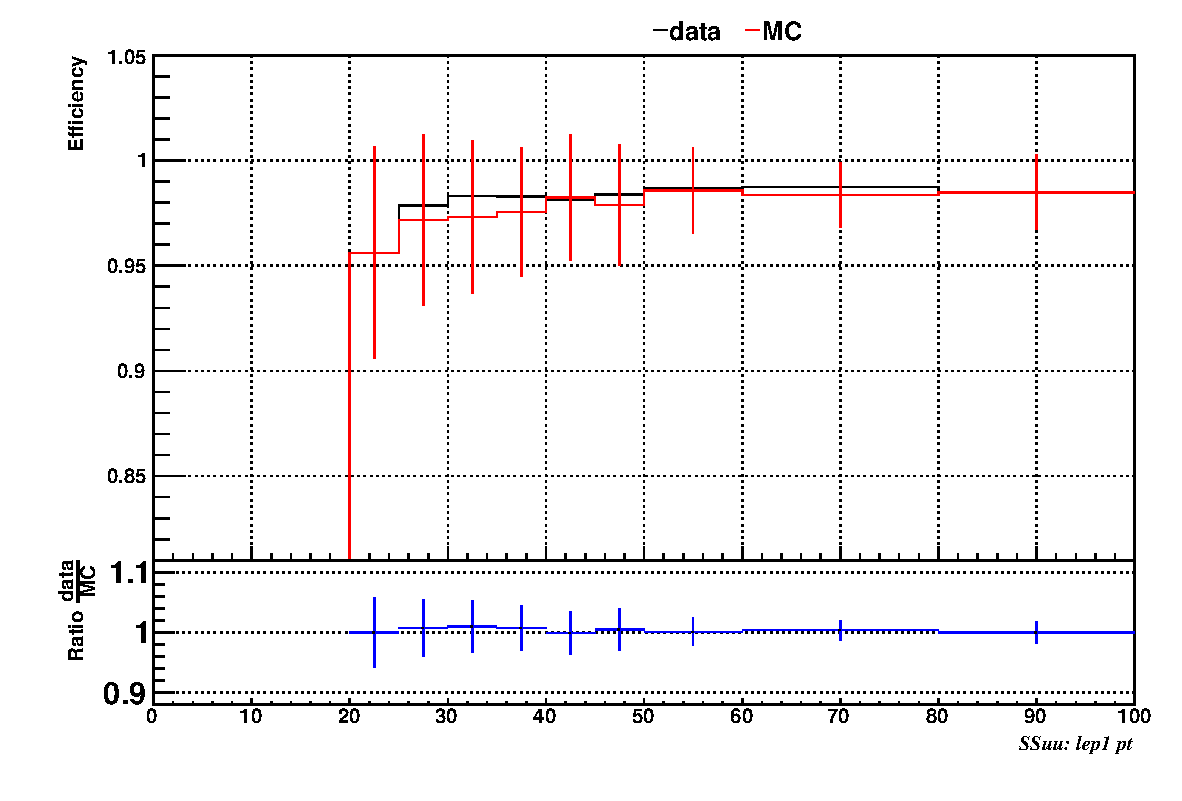
\includegraphics[width=0.49\textwidth]{plots_trigger/1D_eff_lep1_pt_uu_ARCv2_change_3l_pt_ranges.pdf}
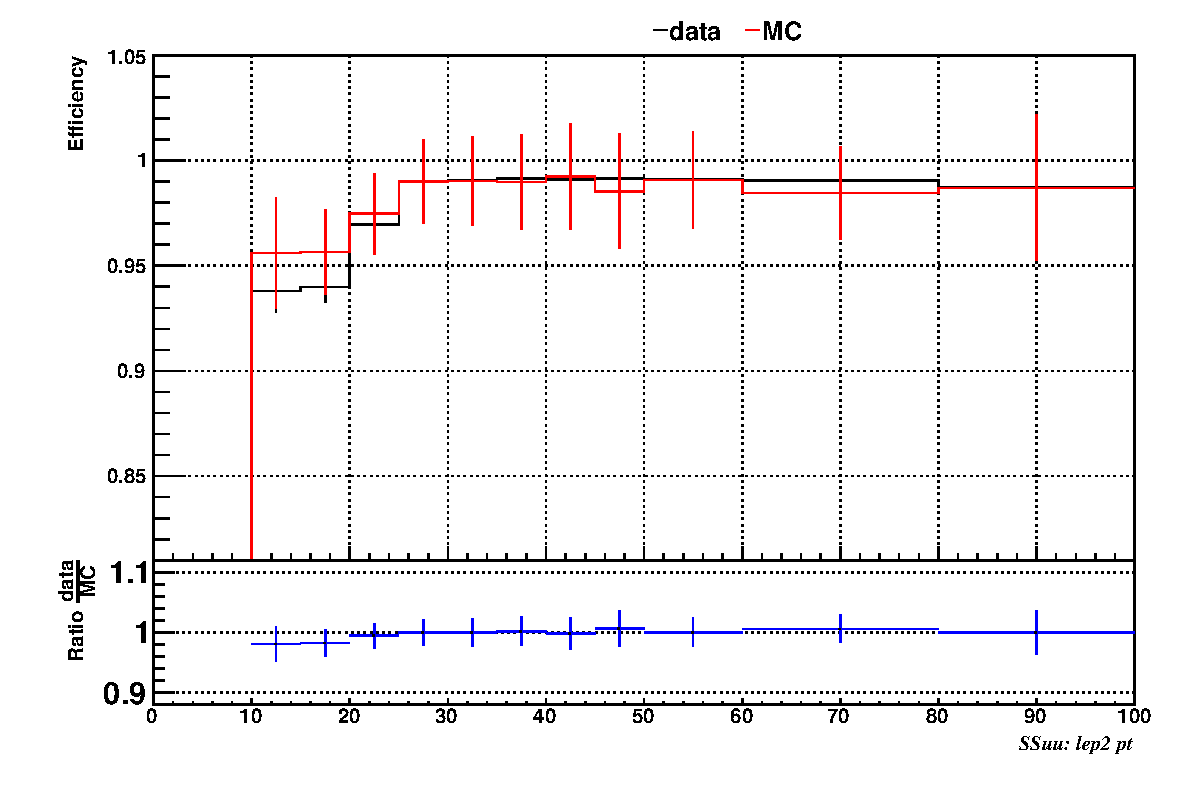
\includegraphics[width=0.49\textwidth]{plots_trigger/1D_eff_lep2_pt_uu_ARCv2_change_3l_pt_ranges.pdf} \\
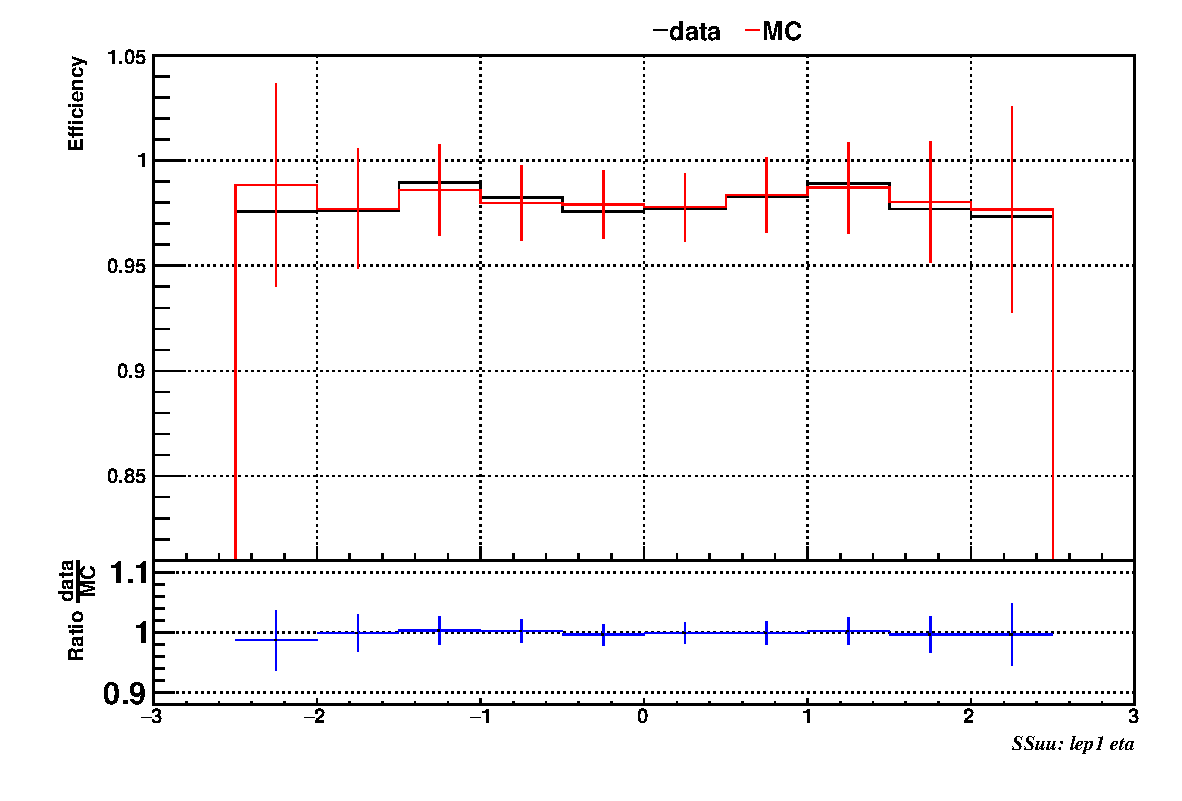
\includegraphics[width=0.49\textwidth]{plots_trigger/1D_eff_lep1_eta_uu_ARCv2_change_3l_pt_ranges.pdf}
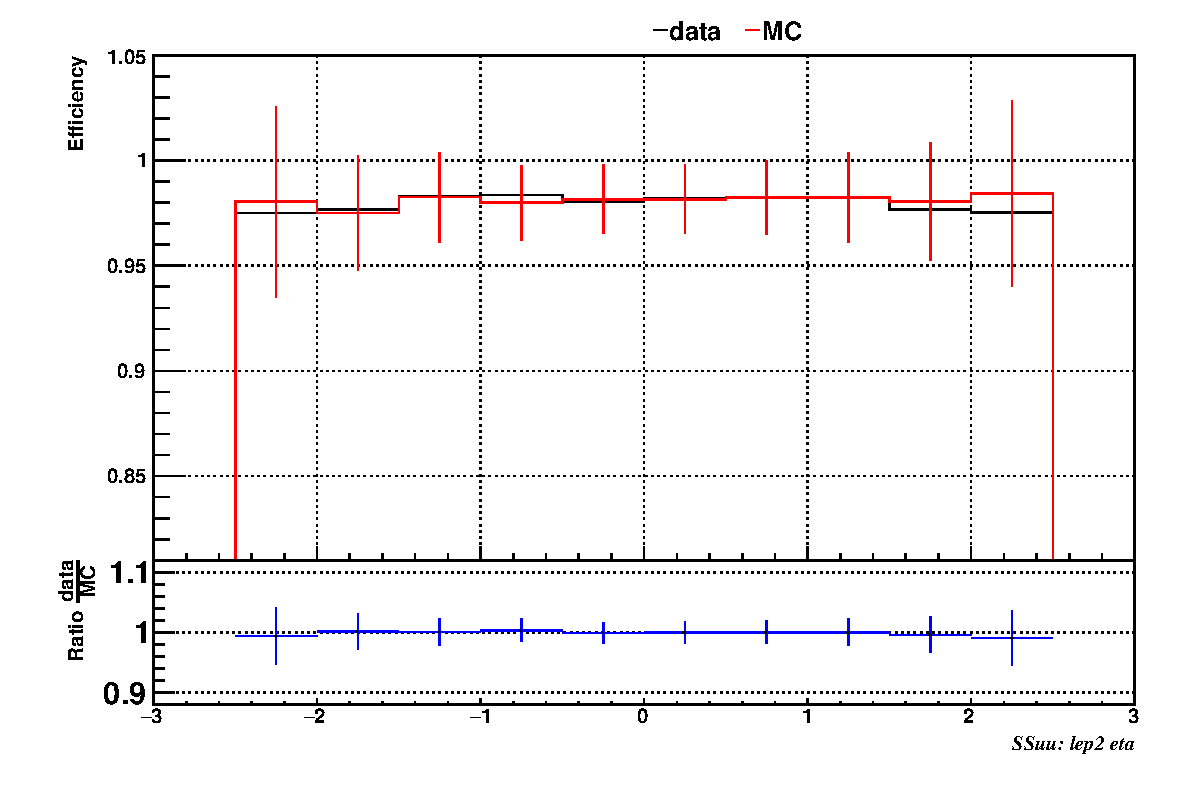
\includegraphics[width=0.49\textwidth]{plots_trigger/1D_eff_lep2_eta_uu_ARCv2_change_3l_pt_ranges.pdf}
\caption{Comparison of the trigger efficiency in the same-sign dimuon category before 
corrections, shown as a function of the \pt and $\eta$ of the leading lepton (left) 
and the sub-leading lepton (right).}
\label{fig:trigeffsmumu}
\end{figure}

\begin{figure}[htp]
\centering
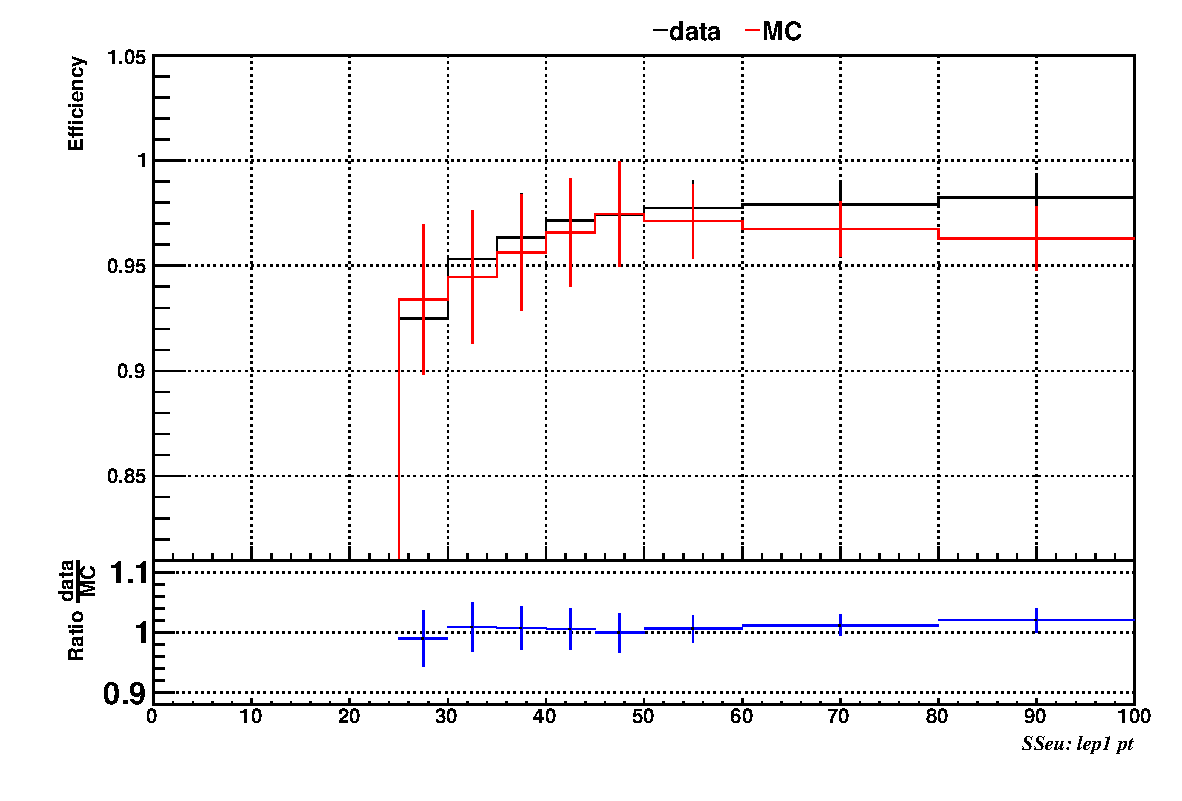
\includegraphics[width=0.49\textwidth]{plots_trigger/1D_eff_lep1_pt_eu_ARCv2_change_3l_pt_ranges.pdf}
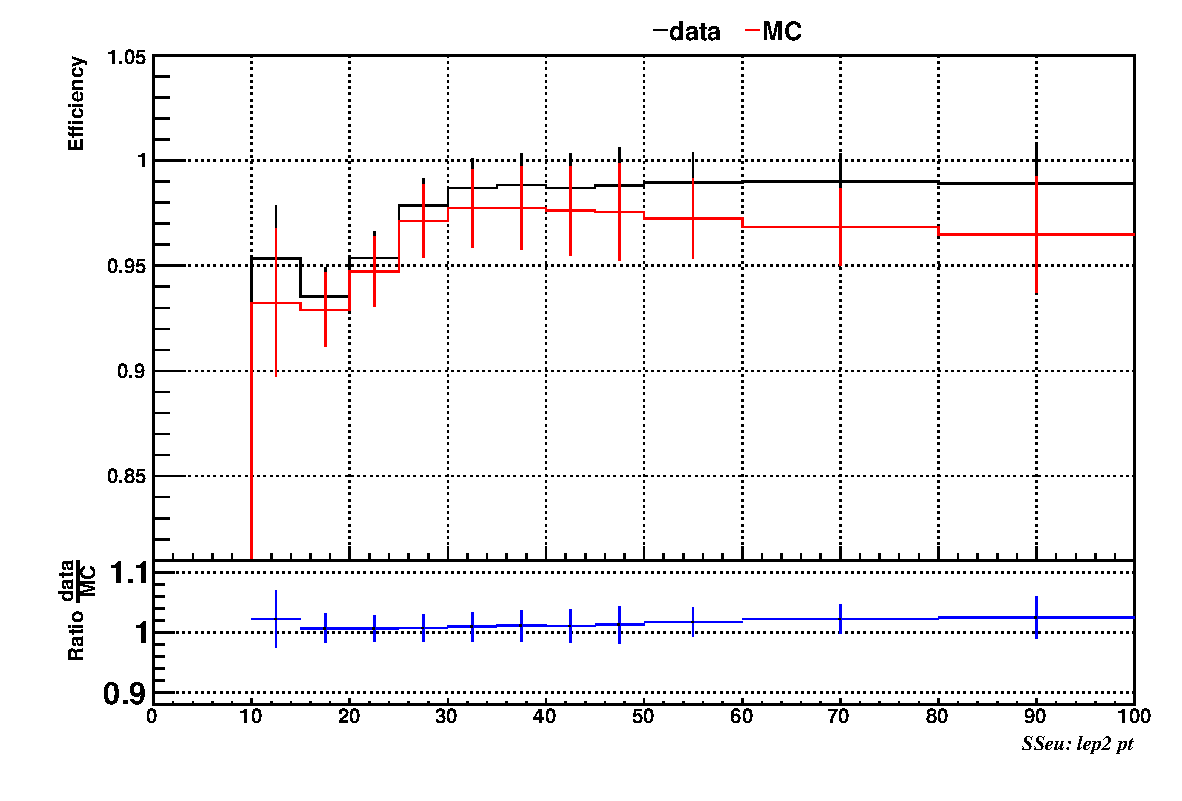
\includegraphics[width=0.49\textwidth]{plots_trigger/1D_eff_lep2_pt_eu_ARCv2_change_3l_pt_ranges.pdf} \\
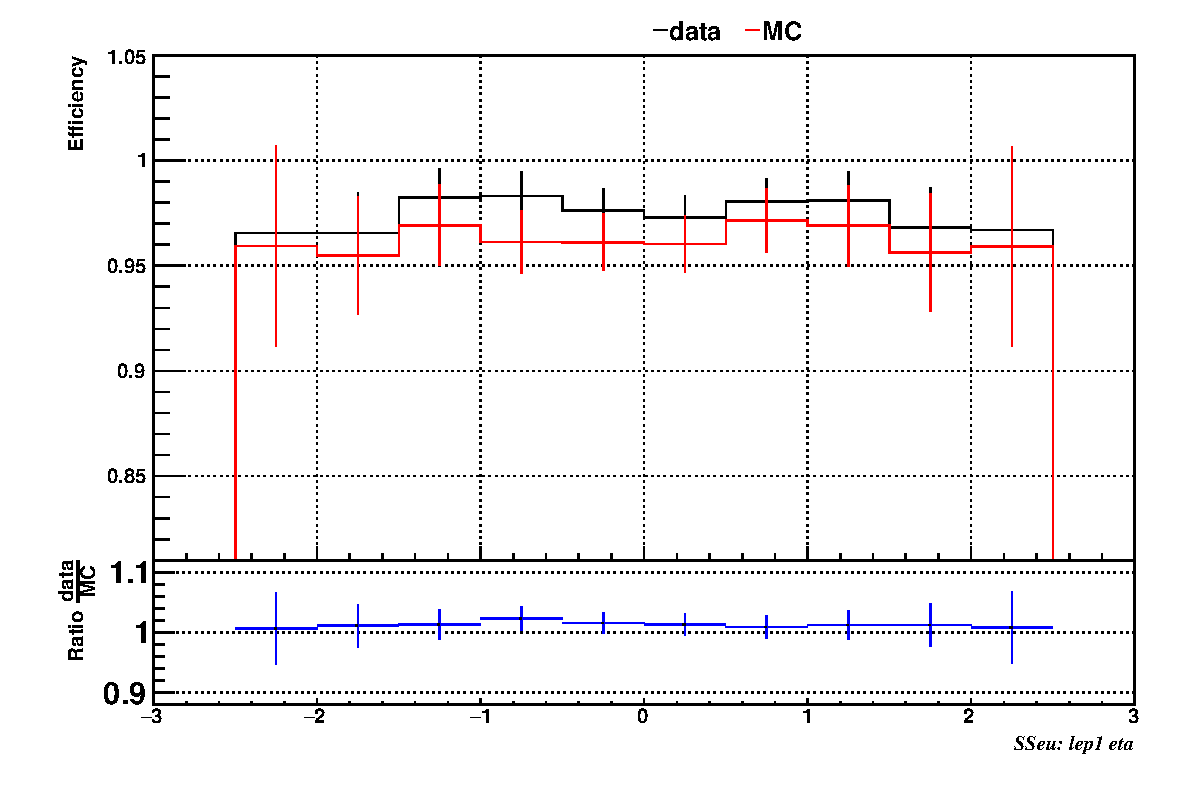
\includegraphics[width=0.49\textwidth]{plots_trigger/1D_eff_lep1_eta_eu_ARCv2_change_3l_pt_ranges.pdf}
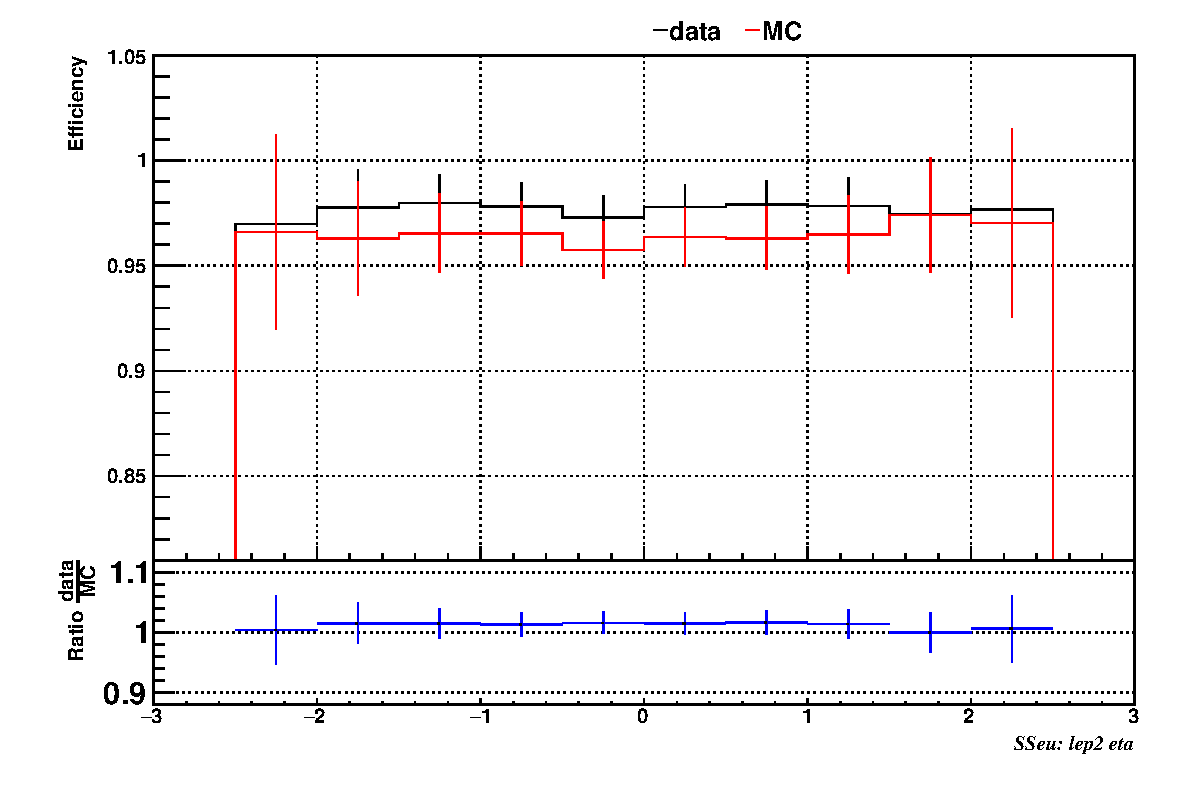
\includegraphics[width=0.49\textwidth]{plots_trigger/1D_eff_lep2_eta_eu_ARCv2_change_3l_pt_ranges.pdf}
\caption{Comparison of the trigger efficiency in the same-sign muon+electron category before 
corrections, shown as a function of the \pt and $\eta$ of the leading lepton (left) 
and the sub-leading lepton (right).}
\label{fig:trigeffsemu}
\end{figure}

\begin{figure}[htp]
\centering
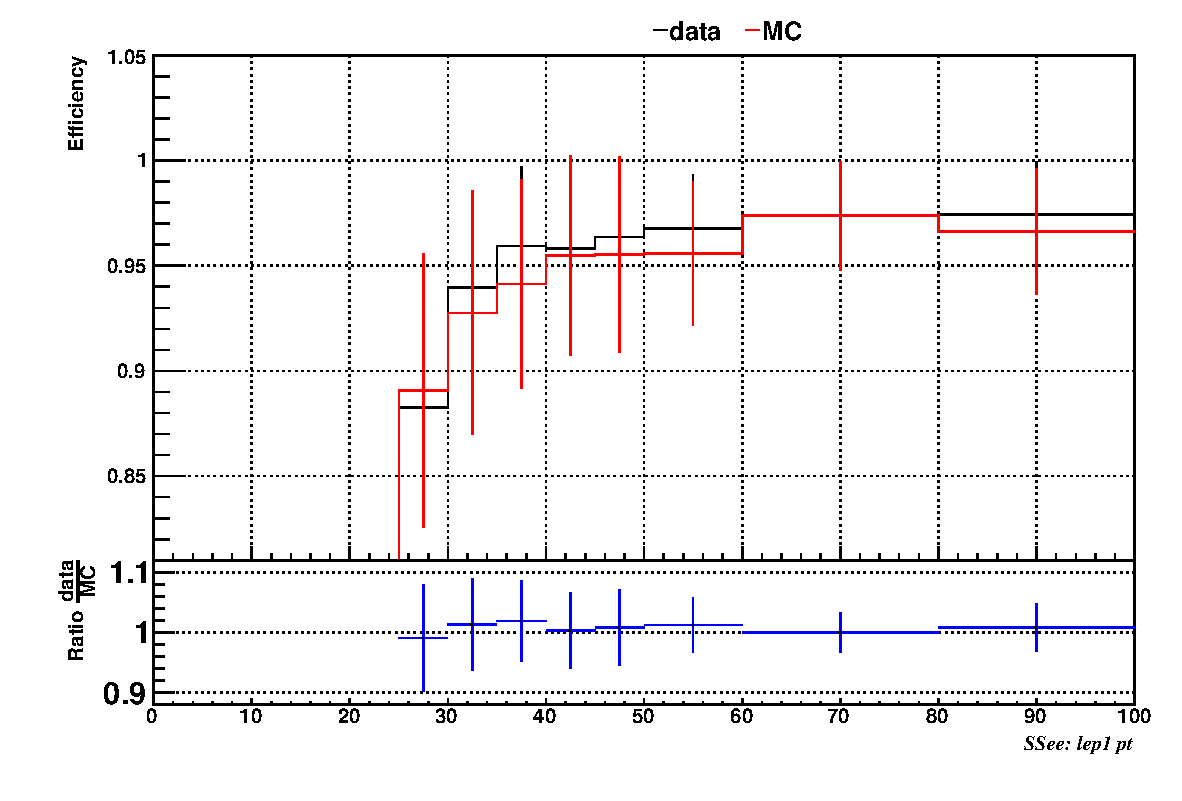
\includegraphics[width=0.49\textwidth]{plots_trigger/1D_eff_lep1_pt_ee_ARCv2_change_3l_pt_ranges.pdf}
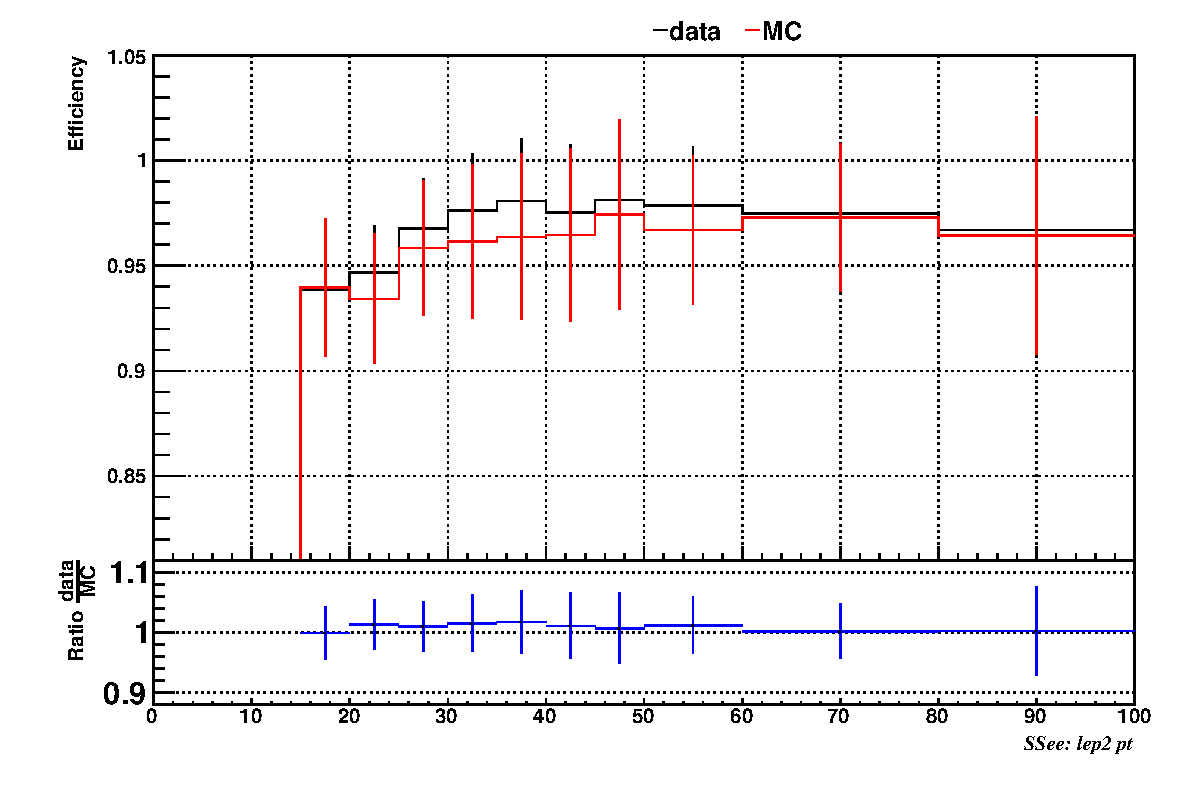
\includegraphics[width=0.49\textwidth]{plots_trigger/1D_eff_lep2_pt_ee_ARCv2_change_3l_pt_ranges.pdf} \\
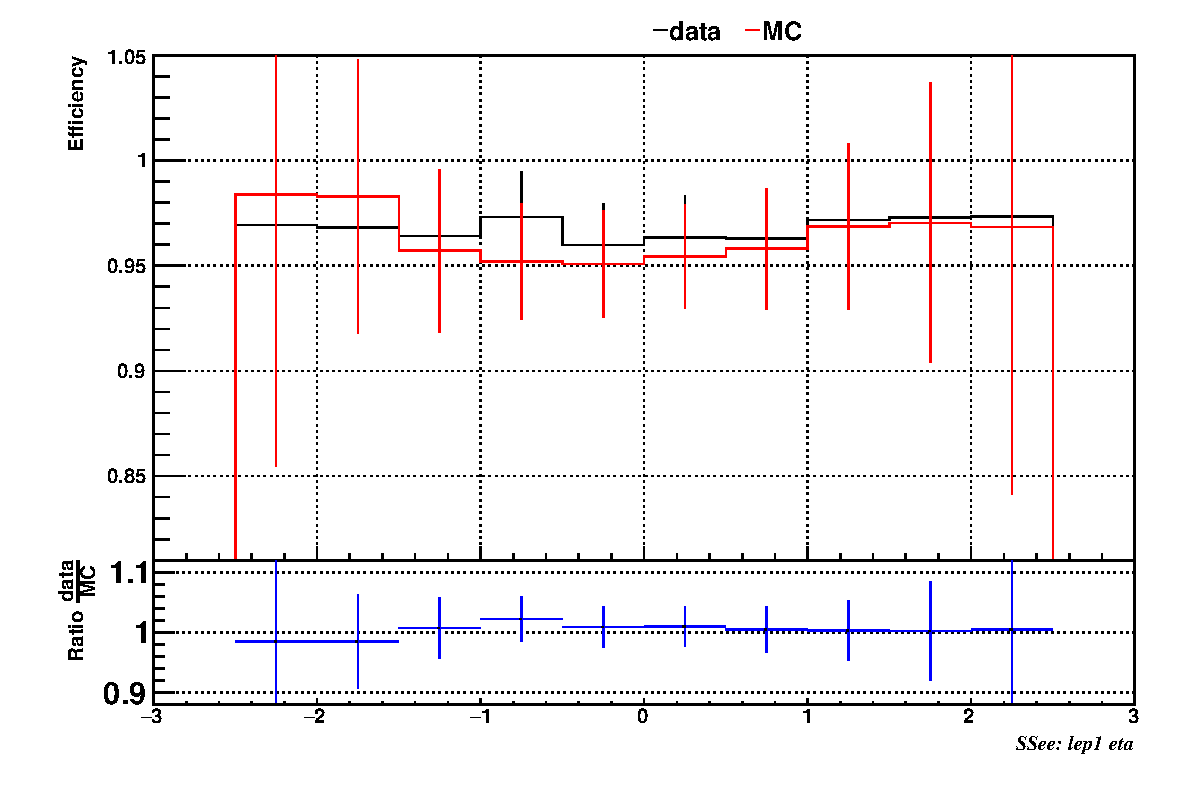
\includegraphics[width=0.49\textwidth]{plots_trigger/1D_eff_lep1_eta_ee_ARCv2_change_3l_pt_ranges.pdf}
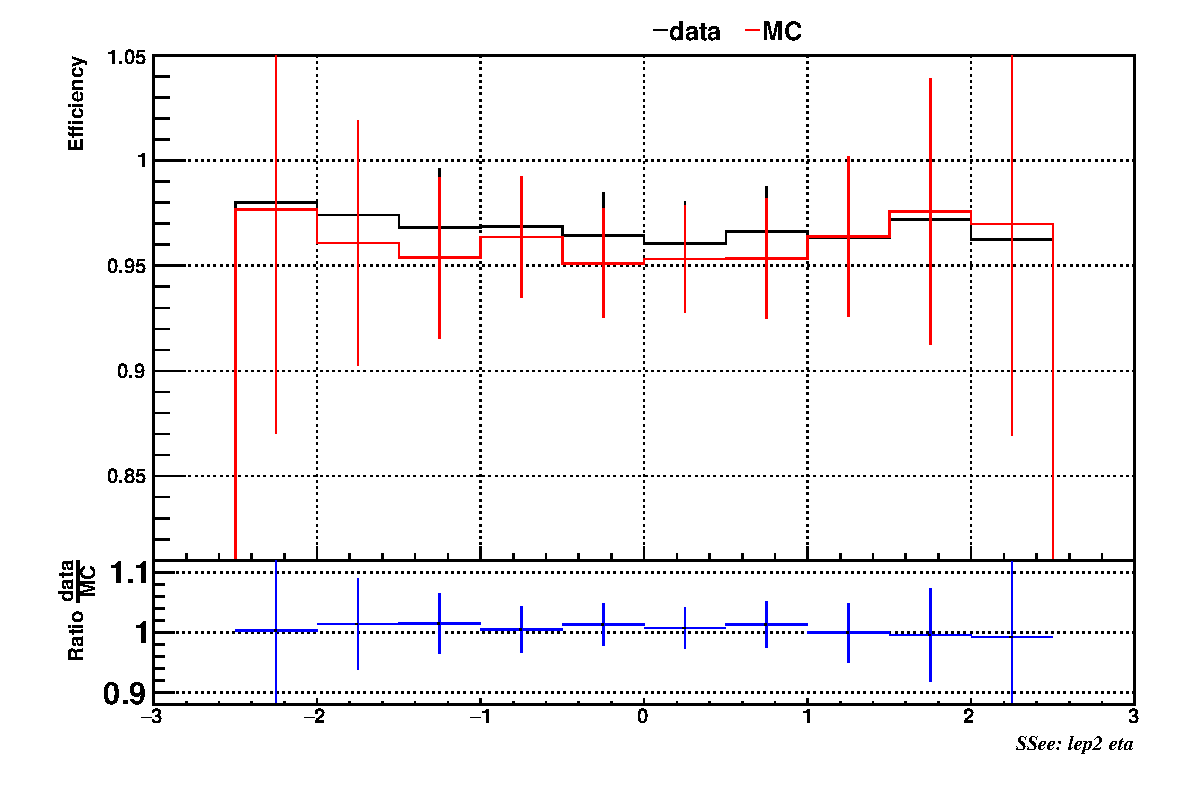
\includegraphics[width=0.49\textwidth]{plots_trigger/1D_eff_lep2_eta_ee_ARCv2_change_3l_pt_ranges.pdf}
\caption{Comparison of the trigger efficiency in the same-sign dielectron category before 
corrections, shown as a function of the \pt and $\eta$ of the leading lepton (left) 
and the sub-leading lepton (right).}
\label{fig:trigeffsee}
\end{figure}

\begin{figure}[htp]
\centering
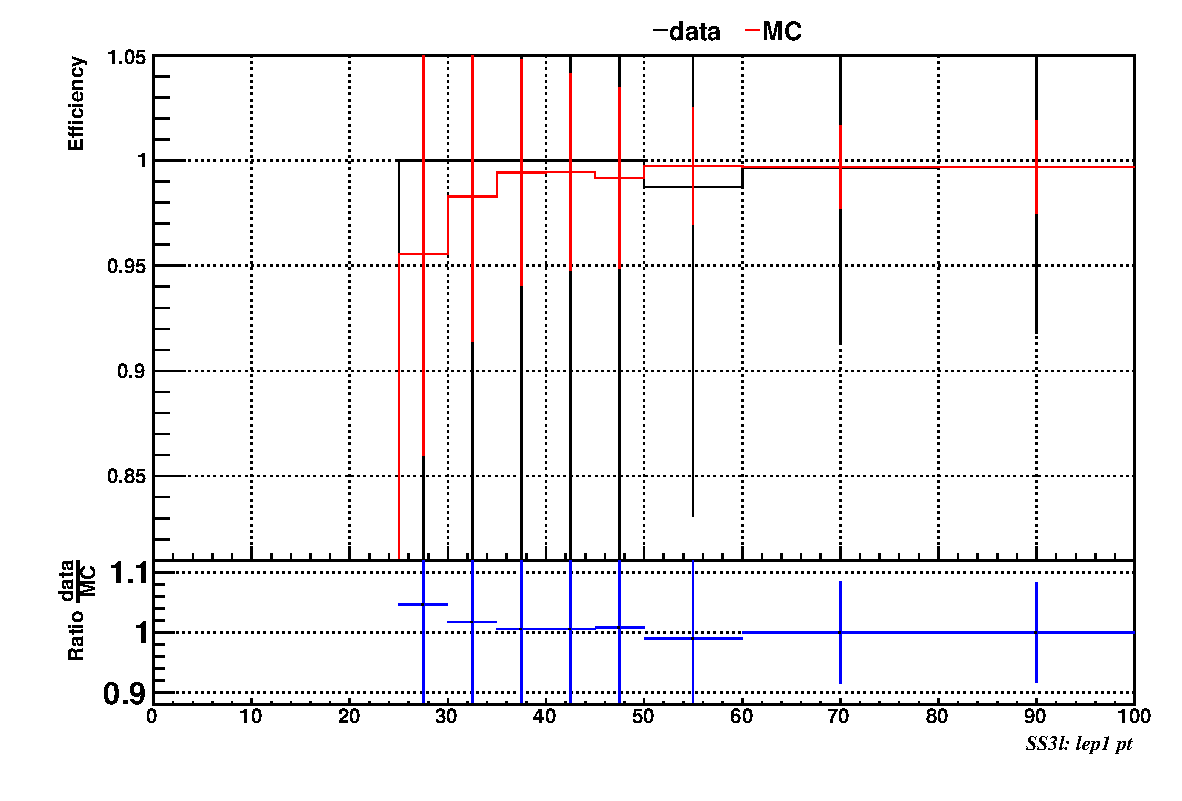
\includegraphics[width=0.49\textwidth]{plots_trigger/1D_eff_lep1_pt_3l_ARCv2_change_3l_pt_ranges.pdf}
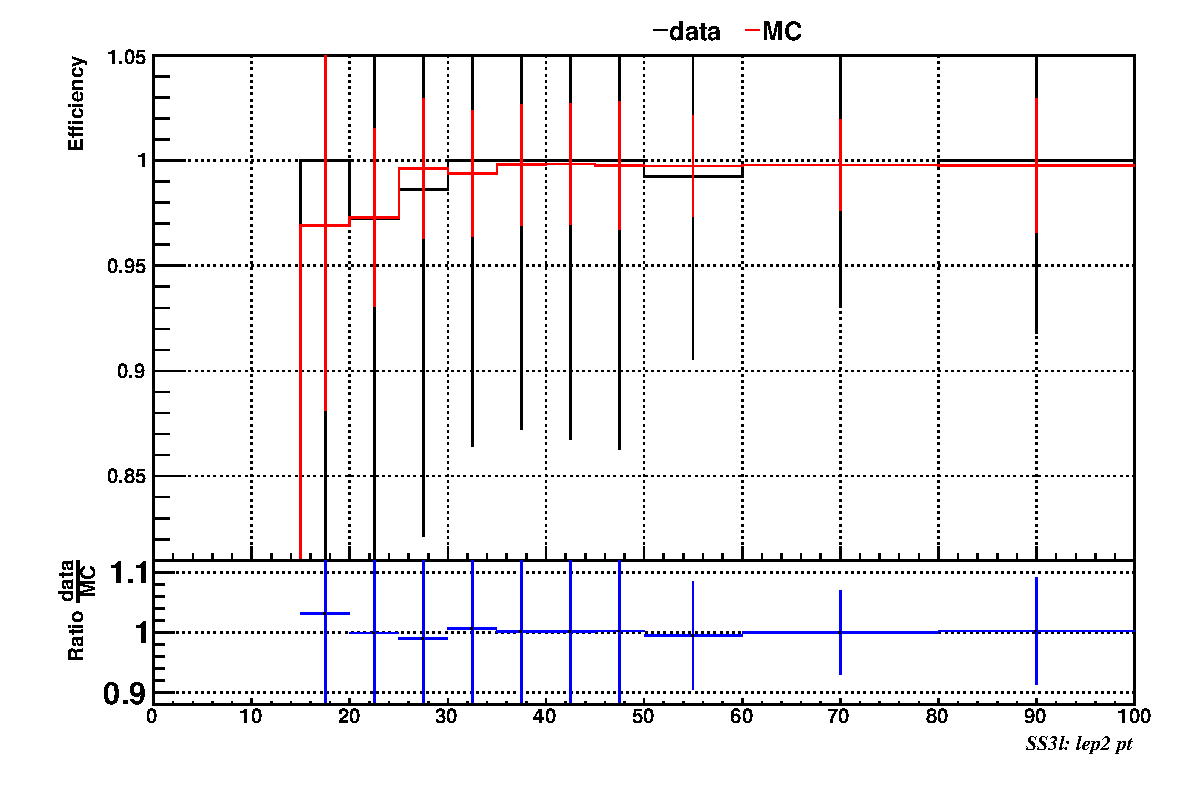
\includegraphics[width=0.49\textwidth]{plots_trigger/1D_eff_lep2_pt_3l_ARCv2_change_3l_pt_ranges.pdf} \\
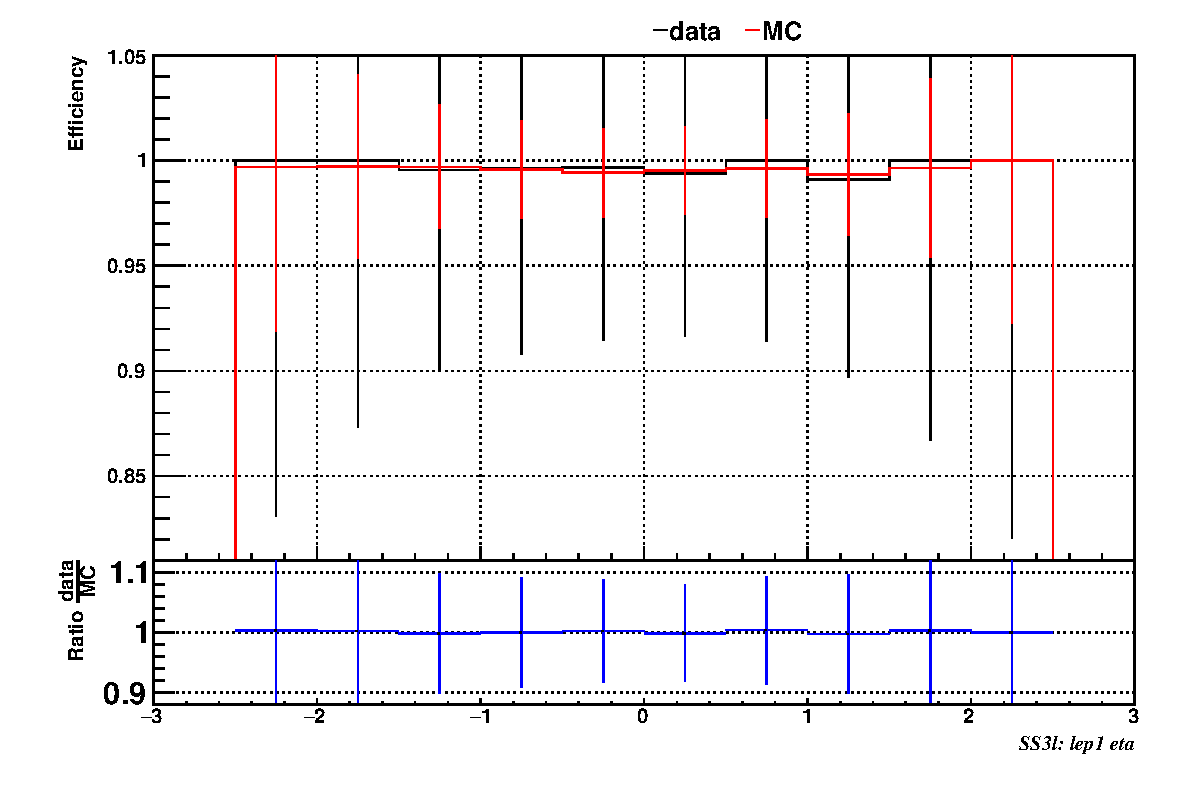
\includegraphics[width=0.49\textwidth]{plots_trigger/1D_eff_lep1_eta_3l_ARCv2_change_3l_pt_ranges.pdf}
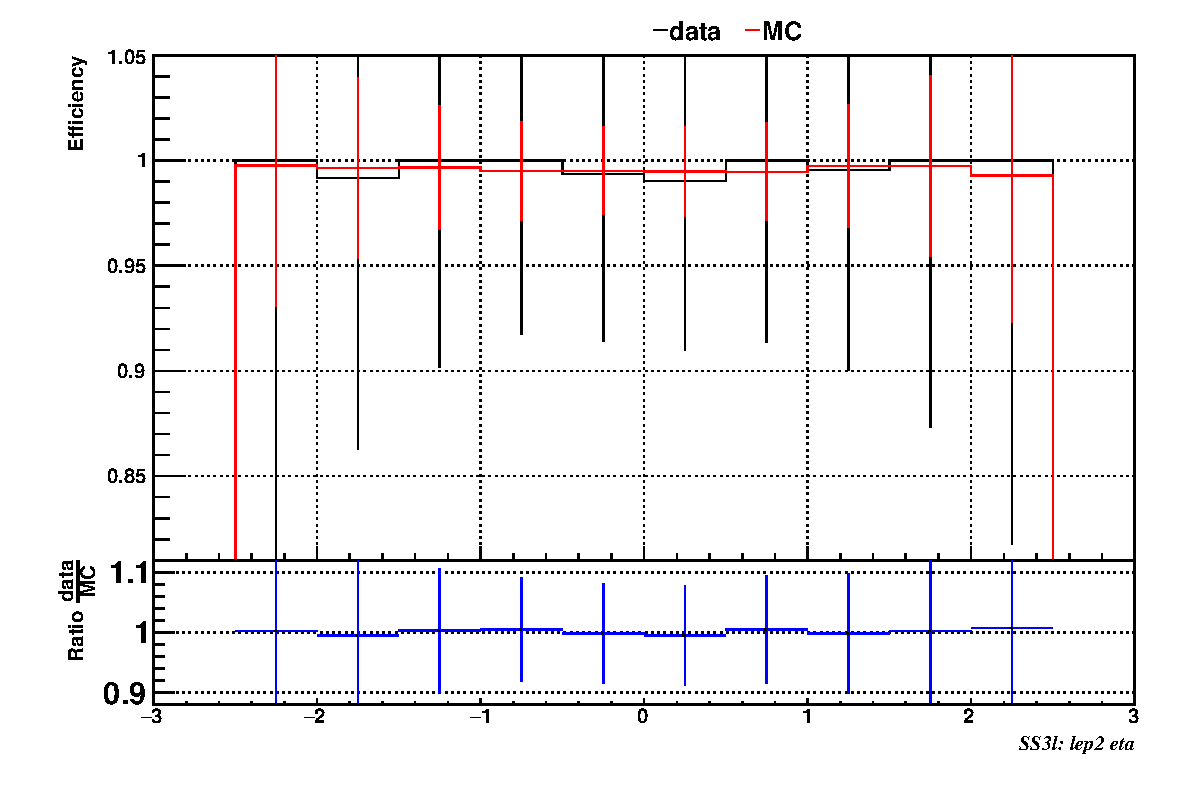
\includegraphics[width=0.49\textwidth]{plots_trigger/1D_eff_lep2_eta_3l_ARCv2_change_3l_pt_ranges.pdf}
\caption{Comparison of the trigger efficiency in the $\geq 3$-lepton category before 
corrections, shown as a function of the \pt and $\eta$ of the leading lepton (left) 
and the sub-leading lepton (right).}
\label{fig:trigeffs3l}
\end{figure}

%\begin{figure}[htp]
%\centering
%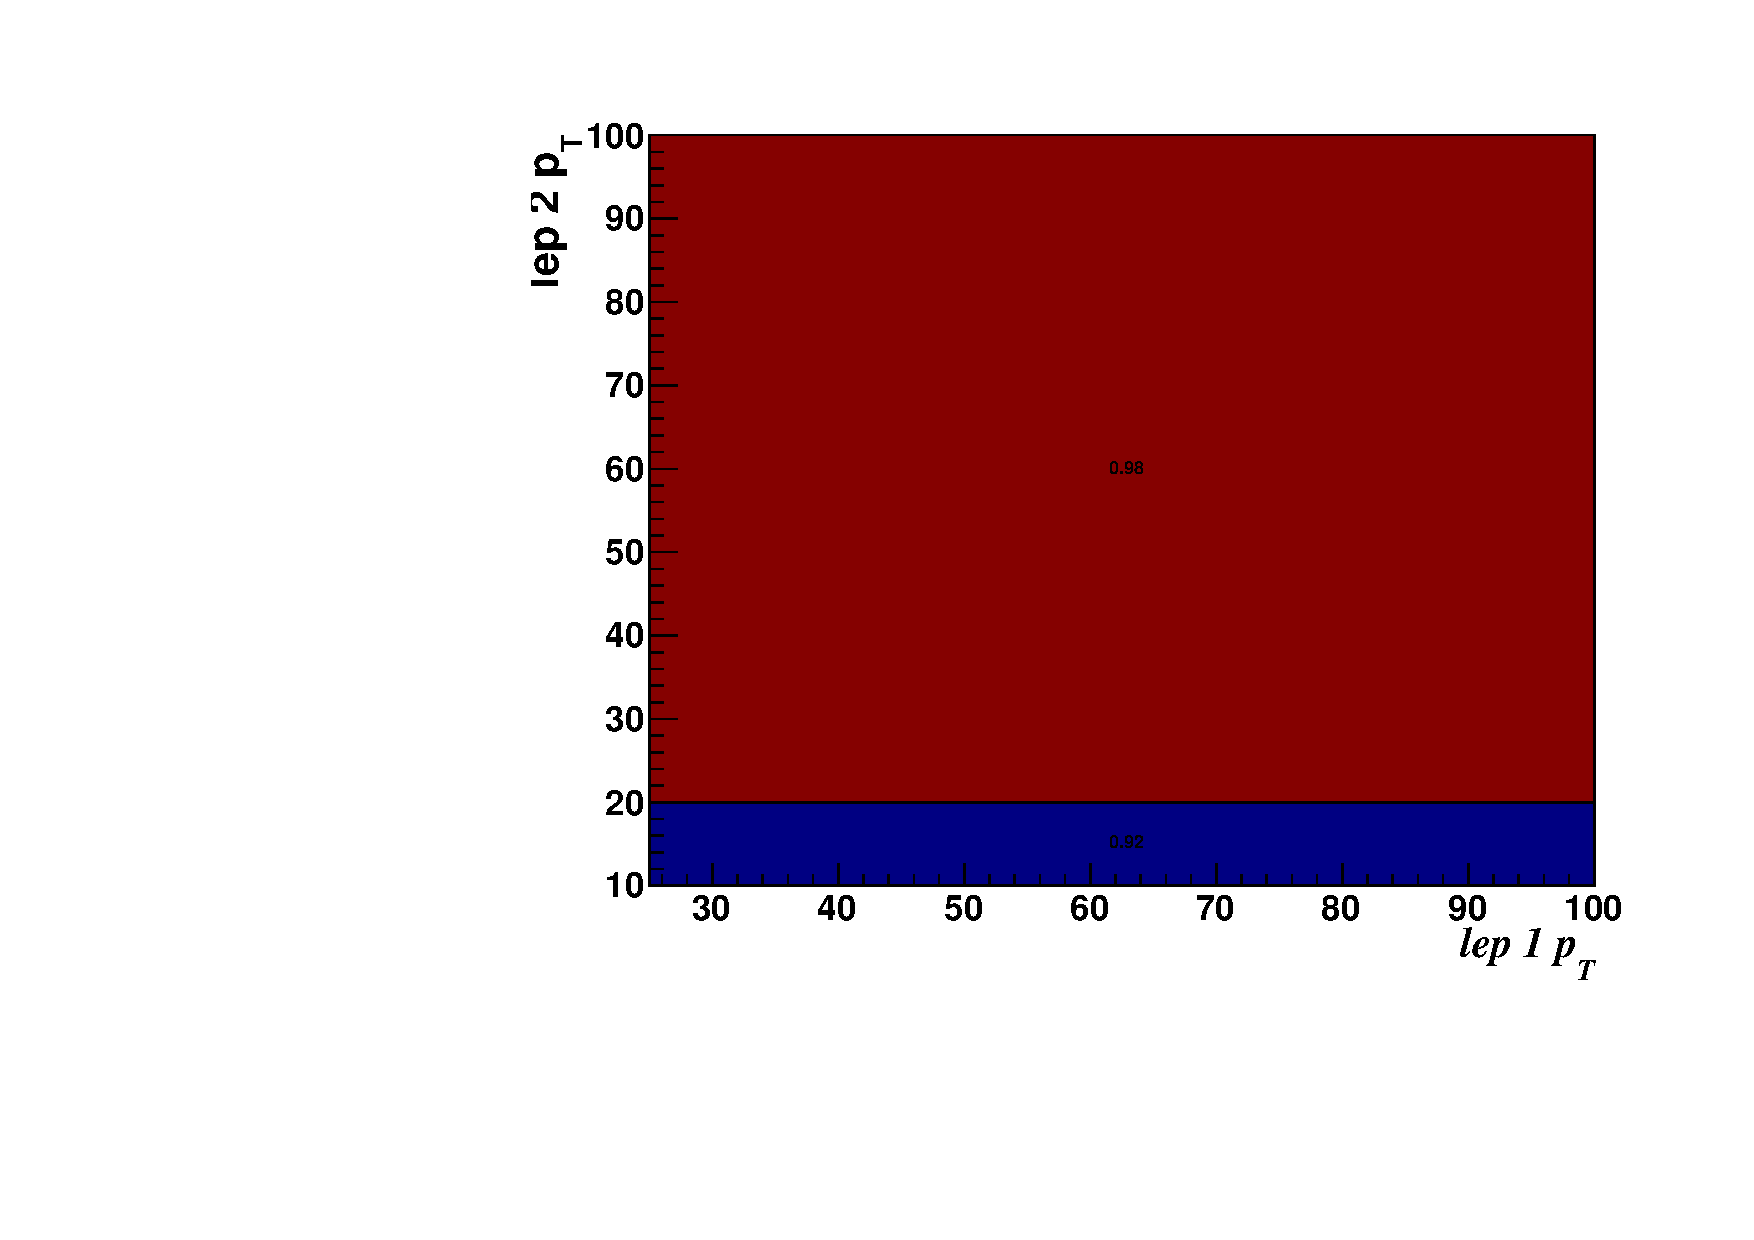
\includegraphics[width=0.49\textwidth]{plots_trigger/trigEffRegions_uu_v2.pdf}
%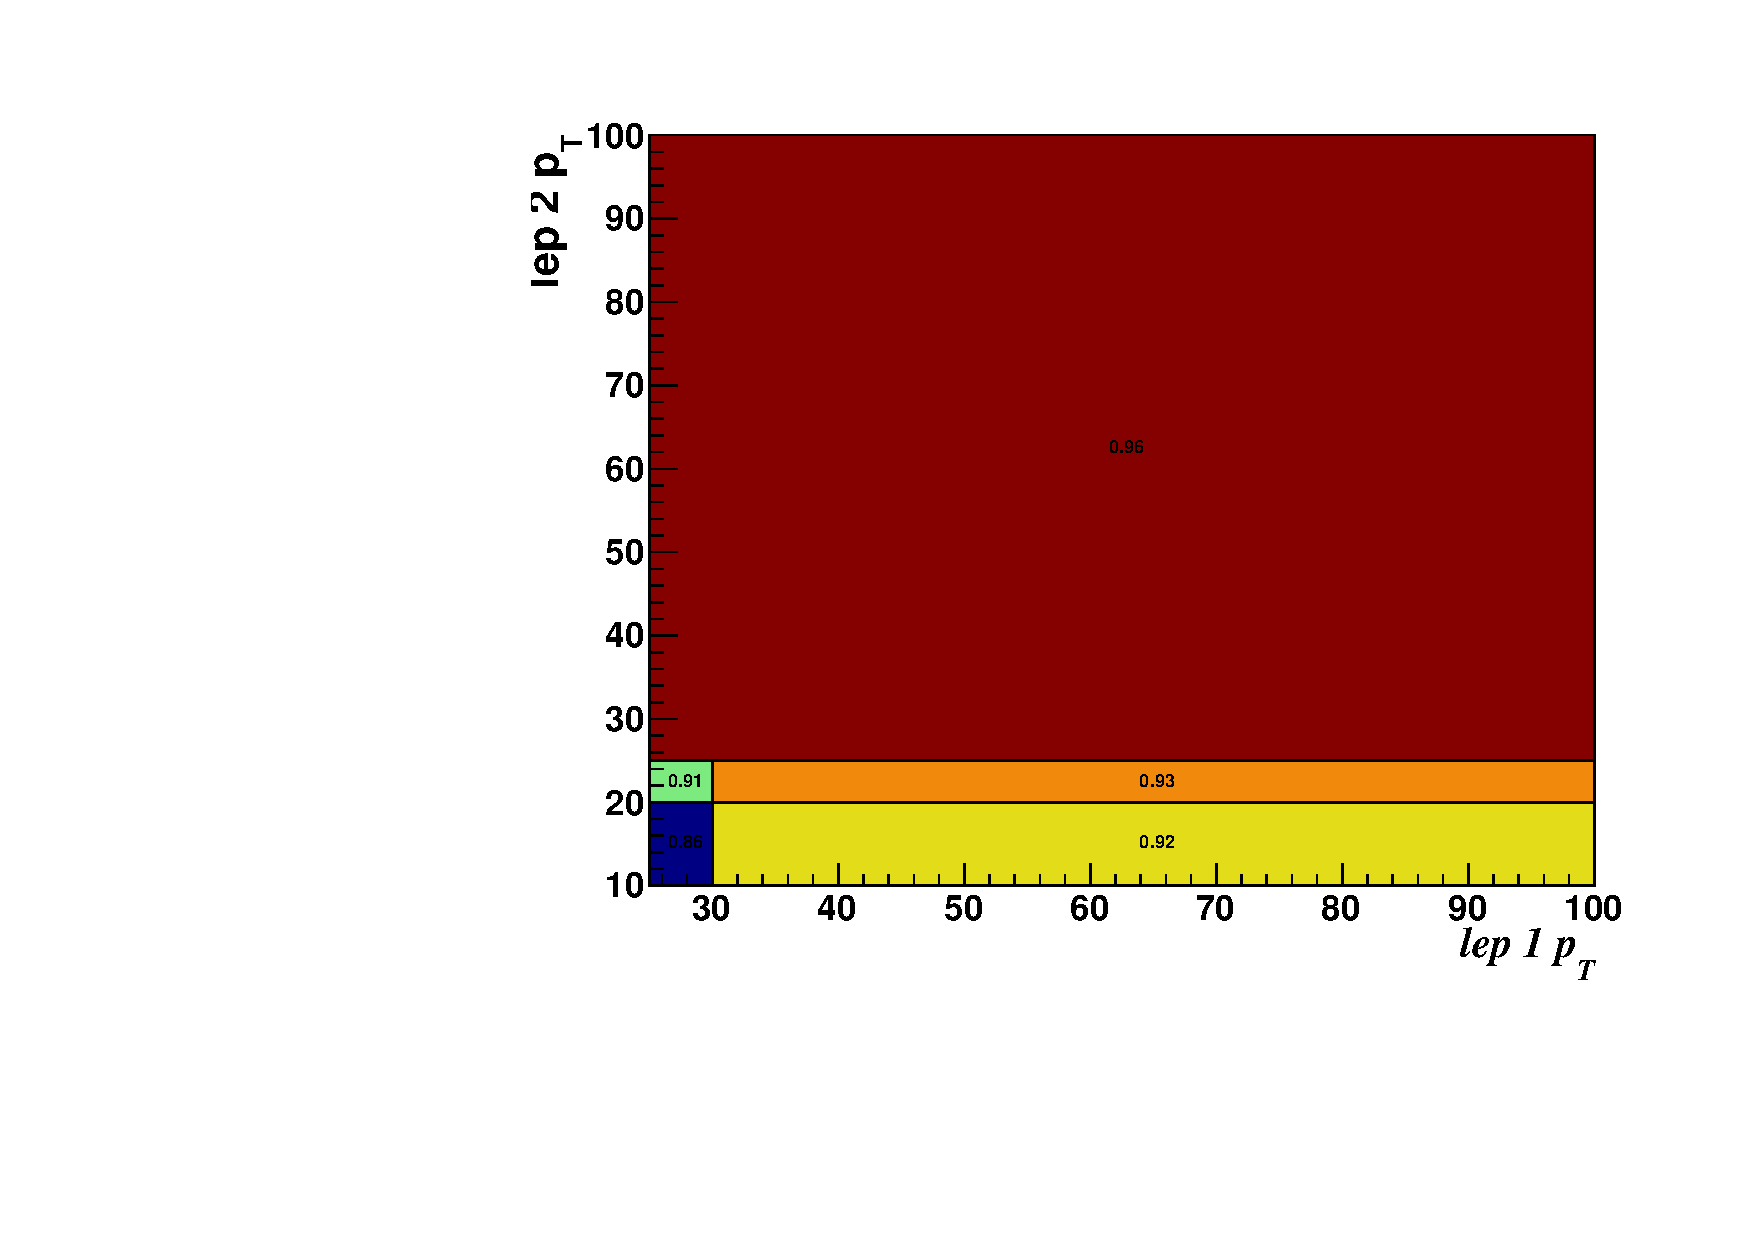
\includegraphics[width=0.49\textwidth]{plots_trigger/trigEffRegions_eu_v2.pdf} \\
%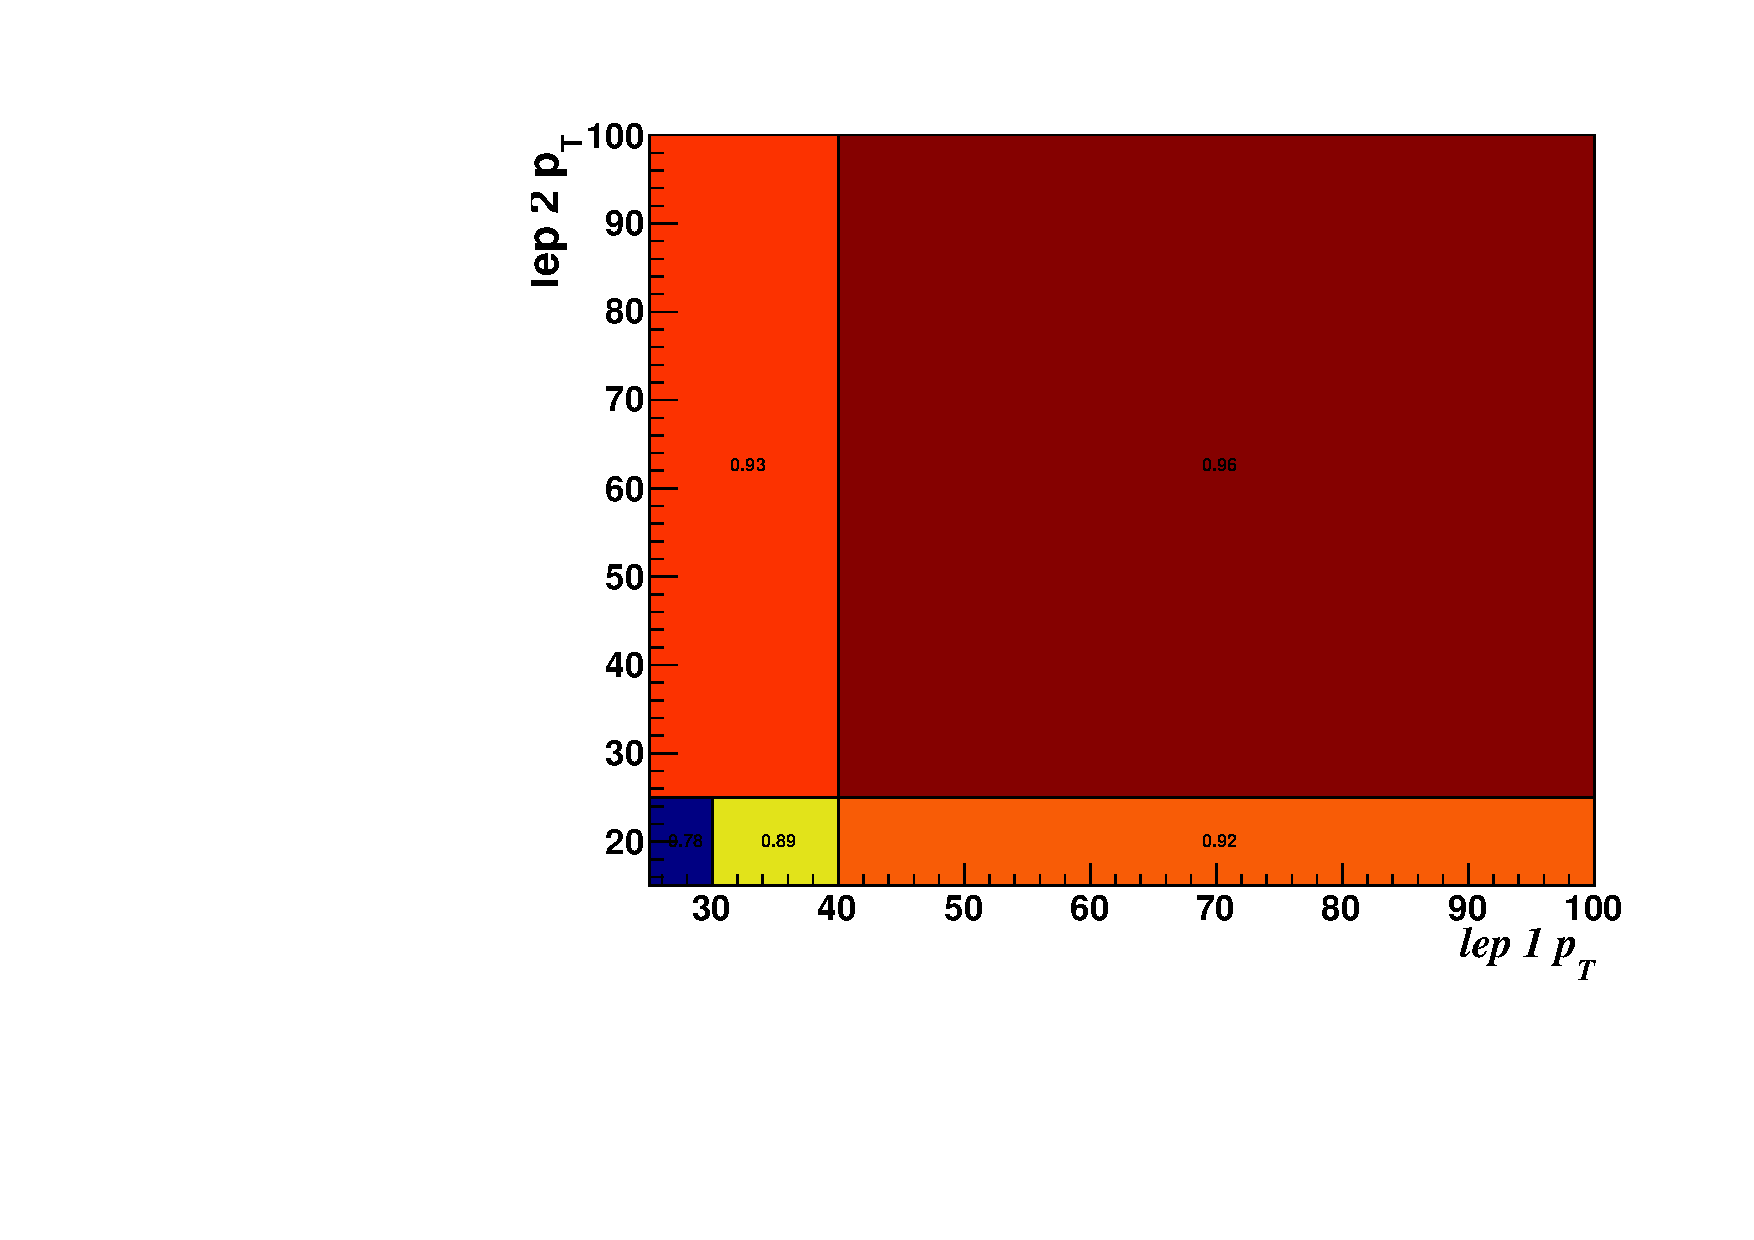
\includegraphics[width=0.49\textwidth]{plots_trigger/trigEffRegions_2e_v2.pdf}
%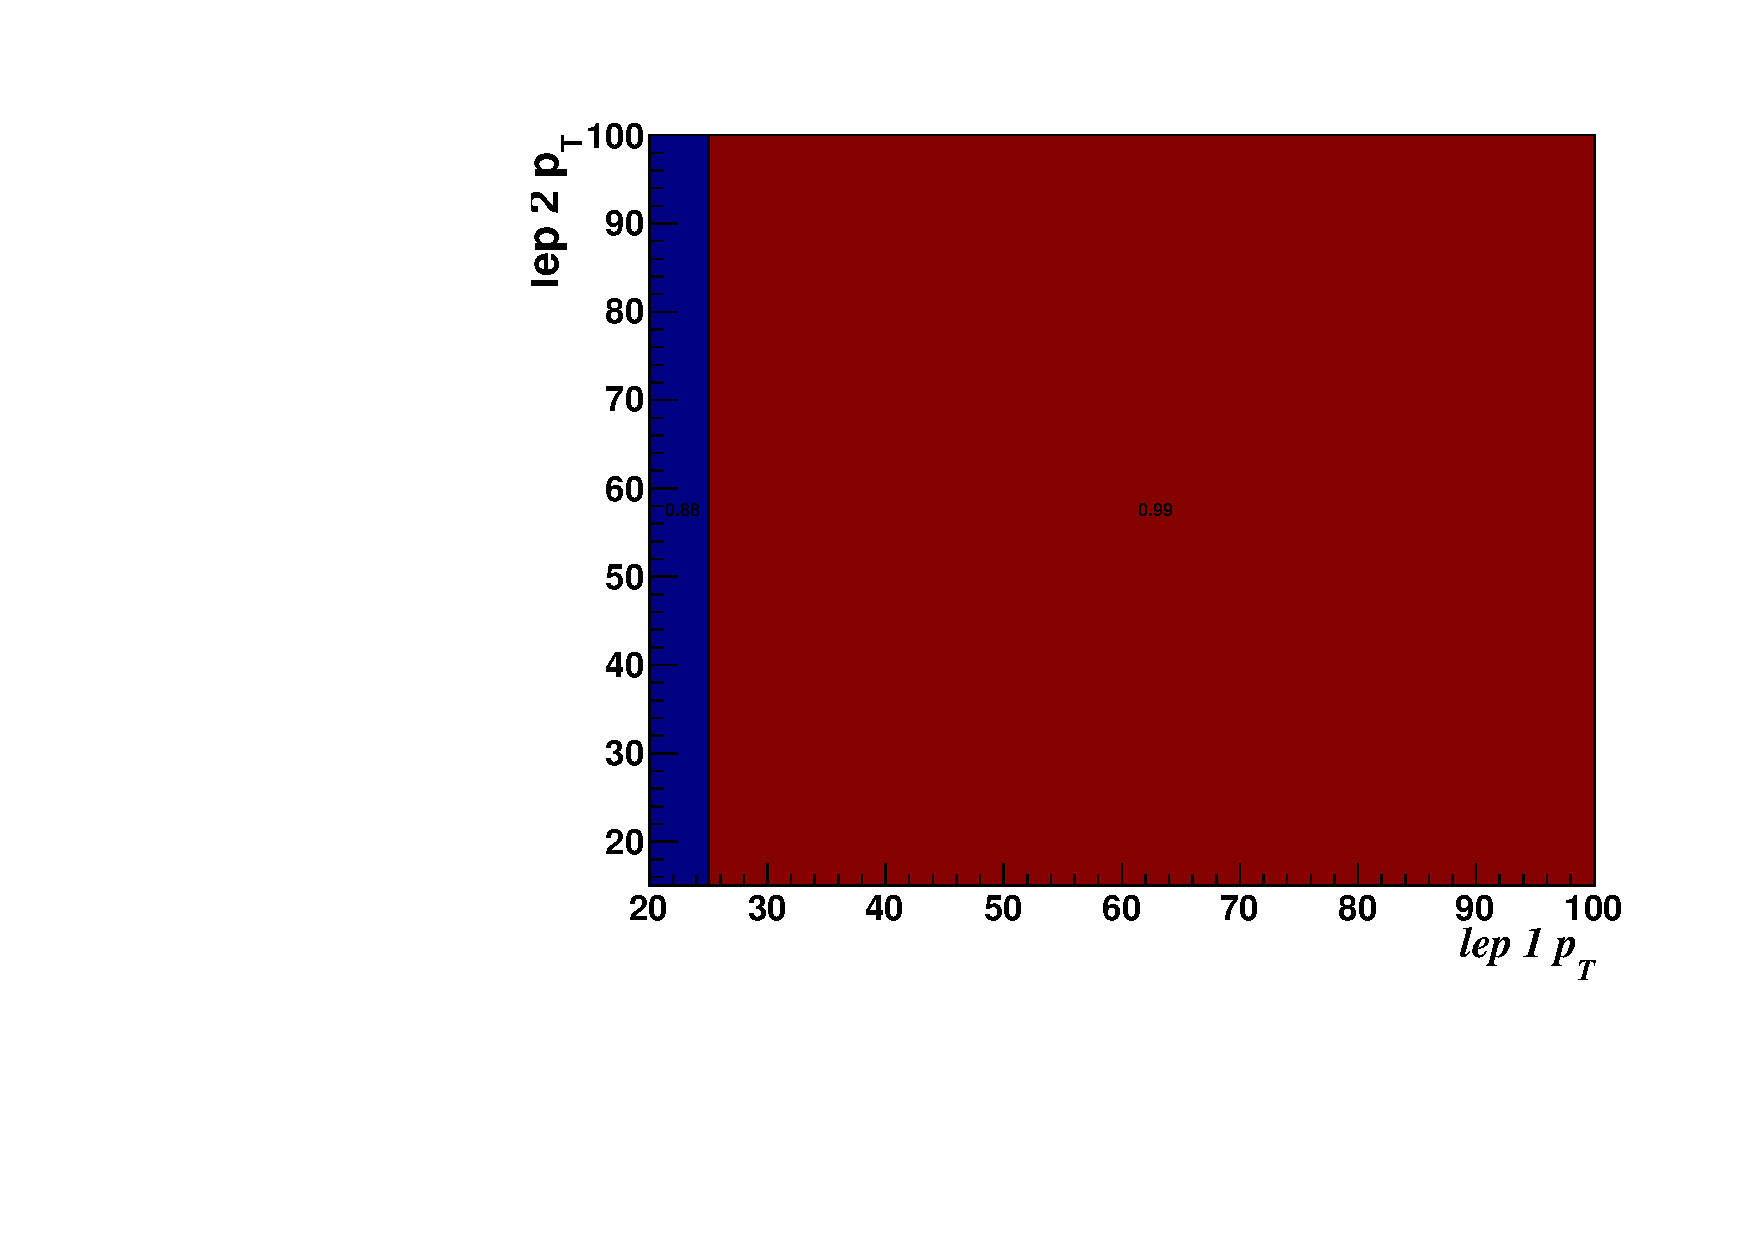
\includegraphics[width=0.49\textwidth]{plots_trigger/trigEffRegions_3l_v2.pdf}
%\caption{Clockwise from top left: trigger efficiency regions in the same-sign dimuon, 
%same-sign muon+electron, 3 lepton and same-sign dielectron categories.}
%\label{fig:trigeffsWeights}
%\end{figure}

%\begin{figure}[htp]
%\centering
%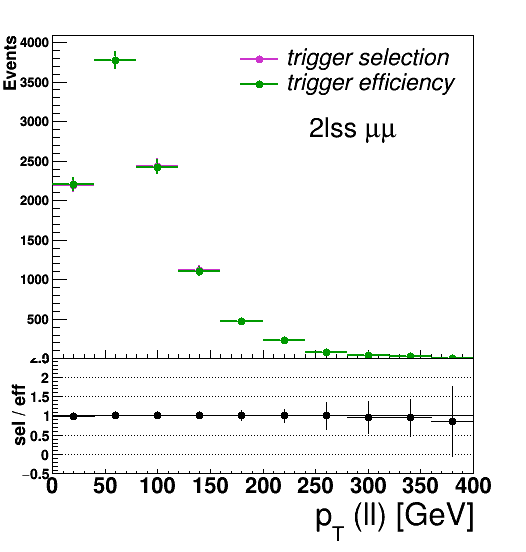
\includegraphics[width=0.32\textwidth]{plots_trigger/dilep_pt_2lss_mm_trg_closure.png}
%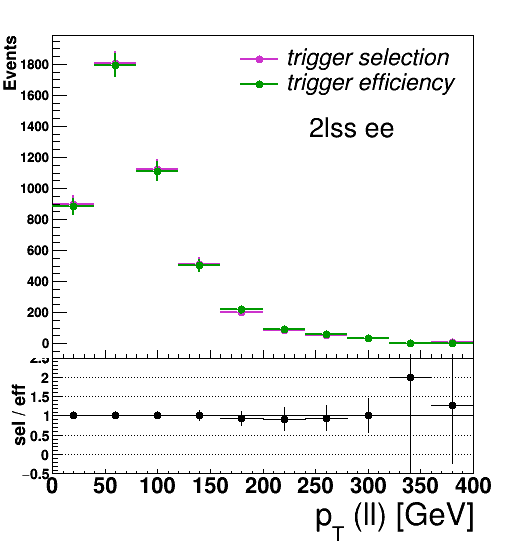
\includegraphics[width=0.32\textwidth]{plots_trigger/dilep_pt_2lss_ee_trg_closure.png}
%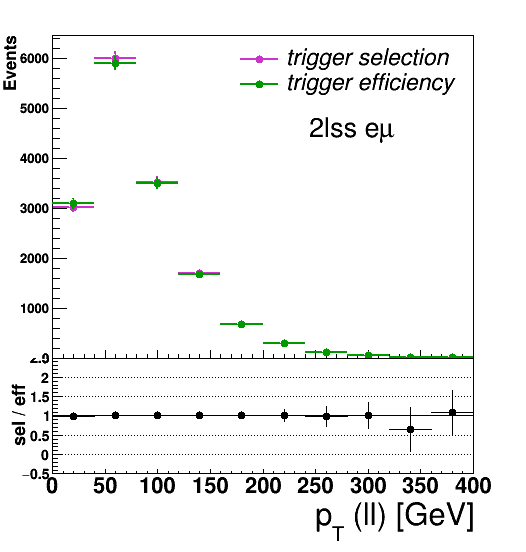
\includegraphics[width=0.32\textwidth]{plots_trigger/dilep_pt_2lss_em_trg_closure.png}\\
%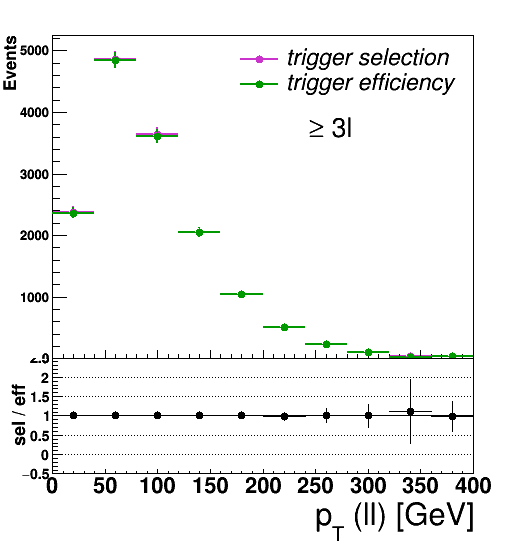
\includegraphics[width=0.32\textwidth]{plots_trigger/dilep_pt_3l_trg_closure.png}
%\caption{Closure test showing the difference between applying the trigger selection directly to ttH MC
%and applying the derived trigger efficiency to ttH MC. Here, the dilepton \pt distribution
%in the 2$\ell$ ($\Pgm\Pgm$, $\Pe\Pe$, $\Pe\Pgm$) categories (top), and the 3$\ell$ category (bottom) is shown.
%Uncertainties are statistical only.}
%\label{fig:trigClosure}
%\end{figure}


\begin{table}
\footnotesize
\centering
\begin{tabular}{l | l}
\hline
Category & Scale Factor \\
\hline
2e & $1.01 \pm 0.02$ \\
e+mu & $1.01 \pm 0.01$ \\
2mu & $1.00 \pm 0.01$ \\
3 and 4l & $1.00 \pm 0.03$ \\
\hline
\end{tabular}
\caption{Trigger efficiency scale factors and associated uncertainties, shown here rounded to the nearest percent.}
\label{tab:trigSFs}
\end{table}

\clearpage
